\documentclass[titlepage,a4paper]{article}

\usepackage{a4wide}
\usepackage[colorlinks=true,linkcolor=black,urlcolor=blue,bookmarksopen=true]{hyperref}
\usepackage{bookmark}
\usepackage{fancyhdr}
\usepackage[spanish]{babel}
\usepackage[utf8]{inputenc}
\usepackage[T1]{fontenc}
\usepackage{graphicx}
\usepackage{float}
\usepackage{listings}
\usepackage[table,xcdraw]{xcolor}
\usepackage{pdfpages}
\newcommand{\codigoMateria}{86.37 / 66.20}
\newcommand{\nombreMateria}{[86.37 / 66.20] Organización de Computadoras}
\newcommand{\curso}{2}
\usepackage{mips}

\newcommand{\numeroTP}{0}
\newcommand{\tituloTP}{Trabajo práctico 0}
\newcommand{\descripcionTP}{Infraestructura básica}

\newcommand{\facultad}{Facultad de Ingeniería}
\newcommand{\universidad}{Universidad de Buenos Aires}
\newcommand{\cuatrimestre}{2do Cuatrimestre de 2020}


\pagestyle{fancy} % Encabezado y pie de página
\fancyhf{}
\fancyhead[L]{TP0 - Infraestructura básica}
\fancyhead[R]{Organización de Computadoras - FIUBA}
\renewcommand{\headrulewidth}{0.4pt}
\fancyfoot[C]{\thepage}
\renewcommand{\footrulewidth}{0.4pt}

\newcommand{\teammember}[3]{
	 #1 & #2 & \texttt{#3}\\
}

\begin{document}
\begin{titlepage} % Carátula
    \centering
      
\includegraphics[scale = 0.75]{images/logo_fiuba.png}\\[1.0 cm]	% Logo universidad
      \textsc{\LARGE \universidad}\\[0.5 cm]	% Nombre universidad
      \textsc{\Large \facultad}\\[0.5 cm]	% Facultad
      \textsc{\large \cuatrimestre}\\[1.0 cm]	% Cuatrimestre
    \centering
    
     \textsc{\Large \nombreMateria}\\[0.5 cm] % Nombre materia
      \textsc{\large Curso \curso}\\[0.4 cm]	% Curso
      
      \rule{\linewidth}{0.2 mm} \\[0.4 cm]
      { \huge \tituloTP}\\[0.5 cm]
      { \huge \bfseries}
      { \huge \bfseries \descripcionTP}\\
      \rule{\linewidth}{0.2 mm} \\[1 cm]
      
     \resizebox{12cm}{!}{
        \begin{tabular}{ | l | l | l | }
          \hline
          Padrón & Alumno & Email \\
          \hline
          \teammember{103442}{Lovera, Daniel}{dlovera@fi.uba.ar}
          \teammember{102914}{More, Agustín}{amore@fi.uba.ar}
          \teammember{99846}{Torresetti, Lisandro}{ltorresetti@fi.uba.ar}
          \hline
      	\end{tabular}
  	}
  	
\end{titlepage}


\tableofcontents % Índice general
\newpage

\lstdefinestyle{customC}{
  language=C,                % choose the language of the code
  backgroundcolor=\color[HTML]{fcfbfc},
  numbers=left,                   % where to put the line-numbers
  stepnumber=1,                   % the step between two line-numbers.        
  numbersep=10pt,                  % how far the line-numbers are from the code
  frame=l,	                   % adds a frame around the code
  showspaces=false,               % show spaces adding particular underscores
  showstringspaces=false,         % underline spaces within strings
  keywordstyle=\color[HTML]{6684e1},
  stringstyle=\color[HTML]{1fad83},     % string literal style
  commentstyle=\color[HTML]{999580},
  showtabs=false,                 % show tabs within strings adding particular underscores
  tabsize=2,                      % sets default tabsize to 2 spaces
  captionpos=b,                   % sets the caption-position to bottom
  breaklines=true,                % sets automatic line breaking
  breakatwhitespace=true,         % sets if automatic breaks should only happen at whitespace
  title=\lstname,                 % show the filename of files included with \lstinputlisting;
  postbreak=\mbox{\textcolor{darkgray}{$\hookrightarrow$}\space},
}

\section{Objetivos}\label{sec:objetivos}
Familiarización de las herramientas de software utilizadas por la cátedra:
\begin{itemize}
\item GCC: Compilador del código fuente.
\item \LaTeX: Herramienta para la generación de documentos.
\item QEMU: Emulador de distintos procesadores sin necesidad de particiones de disco, en particular se trabaja con la arquitectura MIPS.
\end{itemize}

\section{Introducción}\label{sec:intro}
En el presente informe se plantea la resolución de un programa en C que permite la codificación Base64, el programa es controlado por una serie de comandos que permiten seleccionar entre codificación o decodificación así como el origen y el destino de estos datos.

Base64 se creó con el fin de poder transmitir archivos binarios en medios que solo admitían texto, debe su nombre a que 64 es la mayor potencia de 2 que puede ser representada usando únicamente caracteres ASCII imprimibles, los primeros 62 dígitos de la tabla de símbolos corresponden a las letras del alfabeto latino (mayúsculas y minúsculas) y los últimos 2 suelen variar dependiendo del tipo de implementación que se realice, en este trabajo se consideraron los símbolos \verb|+| y \verb|/| como últimos dígitos.

%\section{Programa a implementar}\label{sec:programa_a_implementar}
%Utilizando el lenguaje `C' se implementa un codificador y %decodificador de texto en base64. La entrada será un archivo %especificado en el comando o el \textit{stdin} si ninguno es %especificado, y la salida será otro archivo también especificado en %el comando o el \textit{stdout} si ninguno es especificado.

\section{Detalles de implementación}\label{sec:detalles_implementacion}

\subsection{Base64}
Es un sistema de numeración posicional cuya base es 64 \cite{base64}. Se utilizará para codificar una secuencia de caracteres a un subconjunto de caracteres \verb|ascii|. El proceso de codificación consiste en tomar el texto que se quiere codificar, formar una secuencia de bytes con el equivalente de cada carácter con su valor en binario del código \verb|ascii| \cite{ascii_table}. Por ejemplo en el cuadro \ref{table:paso_1}:

\begin{table}[H]
\centering
\begin{tabular}{l|ccc}
Texto             & C        & o        & s        \\
Equivalente ascii & 67       & 111      & 115      \\
Binario           & 01000011 & 01101111 & 01110011
\end{tabular}
\caption{Texto a binario mediante la codificación ascii}
\label{table:paso_1}
\centering
\end{table}

Una vez obtenida la secuencia de bits (cuya longitud siempre será un múltiplo de ocho), se tomaran cada seis bits (tomándolo de izquierda a derecha), obteniendo el cuadro \ref{table:paso_2}:

\begin{table}[H]
\centering
\setlength{\tabcolsep}{4pt}
\begin{tabular}{l|cccccc||cc|cccc||cccc|cc||cccccc}
Texto             & \multicolumn{8}{c|}{C}        & \multicolumn{8}{c|}{o}        & \multicolumn{8}{c}{s}        \\
Equivalente ascii & \multicolumn{8}{c|}{67}       & \multicolumn{8}{c|}{111}      & \multicolumn{8}{c}{115}      \\
Binario           &0& 1 & 0 & 0 & 0 & 0 & 1 & 1 & 0 & 1 & 1 & 0 & 1 & 1 & 1 & 1 & 0 & 1 & 1 & 1 & 0 & 0 & 1 & 1 \\
Índice & \multicolumn{6}{c||}{16} & \multicolumn{6}{c||}{54} & \multicolumn{6}{c||}{61} & \multicolumn{6}{c}{51}

\end{tabular}
\caption{Reagrupación de bits y conversión a índices}
\label{table:paso_2}
\centering
\end{table}

Como se puede ver en el cuadro \ref{table:paso_2}, cada tres caracteres en el texto original, se generan cuatro secuencias de seis bits completos, esto permite codificar desde secuencias fijas de tres bytes. 

Dado que se toman de a seis bits, el mayor índice será 63 ($2^{6} - 1 = 63$, obteniendo el rango [0, 63] índices posibles). Una vez obtenidos estos índices se mapean a un carácter \verb|ascii| del cuadro \ref{table:equivalencias}.

\begin{table}[H]
\centering
\begin{tabular}{cc|cc|cc|cc}
\rowcolor[HTML]{EAECF0} 
{\color[HTML]{202122} \textbf{Valor}} & {\color[HTML]{202122} \textbf{Carácter}} & {\color[HTML]{202122} \textbf{Valor}} & {\color[HTML]{202122} \textbf{Carácter}} & {\color[HTML]{202122} \textbf{Valor}} & {\color[HTML]{202122} \textbf{Carácter}} & {\color[HTML]{202122} \textbf{Valor}} & {\color[HTML]{202122} \textbf{Carácter}} \\
\rowcolor[HTML]{F8F9FA} 
{\color[HTML]{202122} 0}              & {\color[HTML]{202122} A}                 & {\color[HTML]{202122} 16}             & {\color[HTML]{202122} Q}                 & {\color[HTML]{202122} 32}             & {\color[HTML]{202122} g}                 & {\color[HTML]{202122} 48}             & {\color[HTML]{202122} w}                 \\
\rowcolor[HTML]{F8F9FA} 
{\color[HTML]{202122} 1}              & {\color[HTML]{202122} B}                 & {\color[HTML]{202122} 17}             & {\color[HTML]{202122} R}                 & {\color[HTML]{202122} 33}             & {\color[HTML]{202122} h}                 & {\color[HTML]{202122} 49}             & {\color[HTML]{202122} x}                 \\
\rowcolor[HTML]{F8F9FA} 
{\color[HTML]{202122} 2}              & {\color[HTML]{202122} C}                 & {\color[HTML]{202122} 18}             & {\color[HTML]{202122} S}                 & {\color[HTML]{202122} 34}             & {\color[HTML]{202122} i}                 & {\color[HTML]{202122} 50}             & {\color[HTML]{202122} y}                 \\
\rowcolor[HTML]{F8F9FA} 
{\color[HTML]{202122} 3}              & {\color[HTML]{202122} D}                 & {\color[HTML]{202122} 19}             & {\color[HTML]{202122} T}                 & {\color[HTML]{202122} 35}             & {\color[HTML]{202122} j}                 & {\color[HTML]{202122} 51}             & {\color[HTML]{202122} z}                 \\
\rowcolor[HTML]{F8F9FA} 
{\color[HTML]{202122} 4}              & {\color[HTML]{202122} E}                 & {\color[HTML]{202122} 20}             & {\color[HTML]{202122} U}                 & {\color[HTML]{202122} 36}             & {\color[HTML]{202122} k}                 & {\color[HTML]{202122} 52}             & {\color[HTML]{202122} 0}                 \\
\rowcolor[HTML]{F8F9FA} 
{\color[HTML]{202122} 5}              & {\color[HTML]{202122} F}                 & {\color[HTML]{202122} 21}             & {\color[HTML]{202122} V}                 & {\color[HTML]{202122} 37}             & {\color[HTML]{202122} l}                 & {\color[HTML]{202122} 53}             & {\color[HTML]{202122} 1}                 \\
\rowcolor[HTML]{F8F9FA} 
{\color[HTML]{202122} 6}              & {\color[HTML]{202122} G}                 & {\color[HTML]{202122} 22}             & {\color[HTML]{202122} W}                 & {\color[HTML]{202122} 38}             & {\color[HTML]{202122} m}                 & {\color[HTML]{202122} 54}             & {\color[HTML]{202122} 2}                 \\
\rowcolor[HTML]{F8F9FA} 
{\color[HTML]{202122} 7}              & {\color[HTML]{202122} H}                 & {\color[HTML]{202122} 23}             & {\color[HTML]{202122} X}                 & {\color[HTML]{202122} 39}             & {\color[HTML]{202122} n}                 & {\color[HTML]{202122} 55}             & {\color[HTML]{202122} 3}                 \\
\rowcolor[HTML]{F8F9FA} 
{\color[HTML]{202122} 8}              & {\color[HTML]{202122} I}                 & {\color[HTML]{202122} 24}             & {\color[HTML]{202122} Y}                 & {\color[HTML]{202122} 40}             & {\color[HTML]{202122} o}                 & {\color[HTML]{202122} 56}             & {\color[HTML]{202122} 4}                 \\
\rowcolor[HTML]{F8F9FA} 
{\color[HTML]{202122} 9}              & {\color[HTML]{202122} J}                 & {\color[HTML]{202122} 25}             & {\color[HTML]{202122} Z}                 & {\color[HTML]{202122} 41}             & {\color[HTML]{202122} p}                 & {\color[HTML]{202122} 57}             & {\color[HTML]{202122} 5}                 \\
\rowcolor[HTML]{F8F9FA} 
{\color[HTML]{202122} 10}             & {\color[HTML]{202122} K}                 & {\color[HTML]{202122} 26}             & {\color[HTML]{202122} a}                 & {\color[HTML]{202122} 42}             & {\color[HTML]{202122} q}                 & {\color[HTML]{202122} 58}             & {\color[HTML]{202122} 6}                 \\
\rowcolor[HTML]{F8F9FA} 
{\color[HTML]{202122} 11}             & {\color[HTML]{202122} L}                 & {\color[HTML]{202122} 27}             & {\color[HTML]{202122} b}                 & {\color[HTML]{202122} 43}             & {\color[HTML]{202122} r}                 & {\color[HTML]{202122} 59}             & {\color[HTML]{202122} 7}                 \\
\rowcolor[HTML]{F8F9FA} 
{\color[HTML]{202122} 12}             & {\color[HTML]{202122} M}                 & {\color[HTML]{202122} 28}             & {\color[HTML]{202122} c}                 & {\color[HTML]{202122} 44}             & {\color[HTML]{202122} s}                 & {\color[HTML]{202122} 60}             & {\color[HTML]{202122} 8}                 \\
\rowcolor[HTML]{F8F9FA} 
{\color[HTML]{202122} 13}             & {\color[HTML]{202122} N}                 & {\color[HTML]{202122} 29}             & {\color[HTML]{202122} d}                 & {\color[HTML]{202122} 45}             & {\color[HTML]{202122} t}                 & {\color[HTML]{202122} 61}             & {\color[HTML]{202122} 9}                 \\
\rowcolor[HTML]{F8F9FA} 
{\color[HTML]{202122} 14}             & {\color[HTML]{202122} O}                 & {\color[HTML]{202122} 30}             & {\color[HTML]{202122} e}                 & {\color[HTML]{202122} 46}             & {\color[HTML]{202122} u}                 & {\color[HTML]{202122} 62}             & {\color[HTML]{202122} +}                 \\
\rowcolor[HTML]{F8F9FA} 
{\color[HTML]{202122} 15}             & {\color[HTML]{202122} P}                 & {\color[HTML]{202122} 31}             & {\color[HTML]{202122} f}                 & {\color[HTML]{202122} 47}             & {\color[HTML]{202122} v}                 & {\color[HTML]{202122} 63}             & {\color[HTML]{202122} /}                
\end{tabular}
\caption{Tabla de equivalencias entre caracteres con su equivalente decimal codificado}
\label{table:equivalencias}
\centering
\end{table}

\begin{table}[H]
\centering
\setlength{\tabcolsep}{4pt}
\begin{tabular}{l|cccccc||cc|cccc||cccc|cc||cccccc}
Texto             & \multicolumn{8}{c|}{C}        & \multicolumn{8}{c|}{o}        & \multicolumn{8}{c}{s}        \\
Equivalente ascii & \multicolumn{8}{c|}{67}       & \multicolumn{8}{c|}{111}      & \multicolumn{8}{c}{115}      \\
Binario           &0& 1 & 0 & 0 & 0 & 0 & 1 & 1 & 0 & 1 & 1 & 0 & 1 & 1 & 1 & 1 & 0 & 1 & 1 & 1 & 0 & 0 & 1 & 1 \\
Índice & \multicolumn{6}{c||}{16} & \multicolumn{6}{c||}{54} & \multicolumn{6}{c||}{61} & \multicolumn{6}{c}{51} \\
Codificado & \multicolumn{6}{c||}{Q} & \multicolumn{6}{c||}{2} & \multicolumn{6}{c||}{9} & \multicolumn{6}{c}{z}
\end{tabular}
\caption{Mapeo de índices a caracteres}
\label{table:paso_3}
\centering
\end{table}

Pasando así del texto `\textbf{Cos}' a `\textbf{Q29z}'.

\subsubsection{Caso borde}
Cuando la secuencia a codificar no es múltiplo de tres, no se logran reagrupar los bytes en conjuntos de seis bits, con lo cual, en este caso, se completan con ceros los bits restantes y se procede a codificar de la forma explicada previamente, salvo que los conjuntos de seis bits que queden en cero por la limpieza anterior serán codificadas por el carácter `\textbf{=}'. En cada conjunto de cuatro letras resultantes se pueden obtener {0, 1, 2} caracteres `\textbf{=}' dependiendo de la longitud original del texto a codificar, siguiendo la fórmula $|txt_{codificado}|_{`='} = 3 - |txt_{codificar}|$ donde $|.|$ es la longitud del texto. Ejemplo:

\begin{table}[H]
\centering
\setlength{\tabcolsep}{4pt}
\begin{tabular}{l|cccccc||cc|cccc||cccc|cc||cccccc}
Texto             & \multicolumn{8}{c|}{C}        & \multicolumn{8}{c|}{}        & \multicolumn{8}{c}{}        \\
Equivalente ascii & \multicolumn{8}{c|}{67}       & \multicolumn{8}{c|}{-}      & \multicolumn{8}{c}{-}      \\
 Binario           & 0 & 1 & 0 & 0 & 0 & 0 & 1 & 1 & \cellcolor[HTML]{EAECF0}0 & \cellcolor[HTML]{EAECF0}0 & \cellcolor[HTML]{EAECF0}0 & \cellcolor[HTML]{EAECF0}0 & \cellcolor[HTML]{EAECF0}0 & \cellcolor[HTML]{EAECF0}0 & \cellcolor[HTML]{EAECF0}0 & \cellcolor[HTML]{EAECF0}0 & \cellcolor[HTML]{EAECF0}0 & \cellcolor[HTML]{EAECF0}0 & \cellcolor[HTML]{EAECF0}0 & \cellcolor[HTML]{EAECF0}0 & \cellcolor[HTML]{EAECF0}0 & \cellcolor[HTML]{EAECF0}0 & \cellcolor[HTML]{EAECF0}0 & \cellcolor[HTML]{EAECF0}0 \\
Índice & \multicolumn{6}{c||}{16} & \multicolumn{6}{c||}{48} & \multicolumn{6}{c||}{-} & \multicolumn{6}{c}{-} \\
Codificado & \multicolumn{6}{c||}{Q} & \multicolumn{6}{c||}{w} & \multicolumn{6}{c||}{=} & \multicolumn{6}{c}{=}
\end{tabular}
\caption{Caso borde de codificación}
\label{table:caso_borde}
\centering
\end{table}

En este caso, partiendo de `\textbf{C}' se obtiene `\textbf{Qw==}'. Se puede ver que se cumple con la fórmula, dado que la longitud del texto original $|txt_{codificar}| = 1$ se cumple que la cantidad de iguales en el texto codificado es $|txt_{codificado}|_{`='} = 3 - 1 = 2$.
\newline

Conclusión, la longitud del resultado siempre será múltiplo de cuatro.

Como detalle de implementación, aprovechando las invariantes de la multiplicidad de las longitudes de los textos, se codifican de a bloques de tres caracteres, obteniendo un bloque constante de cuatro caracteres codificados. Además, se arranca de una cadena con cuatro caracteres `=' que serán sobrescritos a medida que se codifica, limitando la ejecución con la fórmula previamente mencionada.


\subsection{Implementación función de codificación}

En primer lugar se leen 3 bytes del archivo pasado por parámetro al programa y se los almacena en un \textit{buffer}, luego este es pasado a la función \textit{combineBytes} para obtener un código binario de los bytes leídos. A continuación se muestra el código de dicha función:

\begin{lstlisting}[style=customC]
int combineBytes(char* block, size_t readBytes, bool code){
	int resultado = (0x00000000);
	int SHIFTS = 24;
	int mult = (code) ? 8 : 6;
	for (int i = 0; i < readBytes; i++){
		int shiftLeft = SHIFTS - (i + 1) * mult;
		int toShift = (code) ? (int)block[i] : findPosition(block[i]);
		if (toShift < 0){
			fprintf(stderr, "Error: El caracter %c no se encuentra en base 64\n", block[i]);
			return -1;
		}
		resultado |= toShift << shiftLeft;
	}
	return resultado;
}
\end{lstlisting}

El parámetro \textit{code} es un booleano que sirve para saber si tenemos que codificar o decodificar el buffer. Dado que en ambos casos se debe realizar un shift a izquierda primero de cierta cantidad de bits para alinearlos de manera correcta y que sea trivial la separación en la codificación. Se encontró una relación para hacerlo, la misma es la siguiente: $$ 24 - (i + 1) * mult $$

En caso de estar codificando \verb|mult| debe valer 8 y en caso contrario 6. Luego realizamos un \verb|loop| en el cual la cantidad de iteraciones está dada por la cantidad de bytes leídos anteriormente. En cada iteración la cantidad de bits a desplazar hacia la izquierda se va adaptando hasta que no sea necesario un nuevo desplazamiento, así obtenemos el código binario de manera correcta. \newline

La variable \textit{toShift} contiene un entero que representa el código ASCII o el código en Base64, en caso de estar decodificando y que el carácter no se encuentre en la tabla de símbolos de Base64, \textit{findPosition} devolverá -1 lo cual hará que la sentencia del \verb|if| sea verdadera y se imprimirá el mensaje por \textit{stderr}.\newline

En caso de que no haya ningún error, la ejecución continua y se realiza el shift correspondiente. \newline

Una vez que la función devuelve el código binario de los bytes leídos del archivo se pasa el resultado a la función \textit{codification}:

\begin{lstlisting}[style=customC]
char* codification(int binaryCode, size_t readBytes){
	int shiftsLeft[] = {8, 14, 20, 26};
	int shiftRight = 26;
	char* code = malloc(5);
	code[0] = '=';
	code[1] = '=';
	code[2] = '=';
	code[3] = '=';
	code[4] = '\0';
	size_t posCode = 0;
	for (size_t i = 0; i < readBytes + 1; i++){
		int binaryCodeAux = binaryCode; //Para no modificar el codigo binario original
		binaryCodeAux = binaryCodeAux << shiftsLeft[i];
		binaryCodeAux = (int)((unsigned) binaryCodeAux >> shiftRight);
		code[posCode++] = BASE64[binaryCodeAux];
	}
	return code;
}
\end{lstlisting}

Primero se utiliza memoria dinámica para crear un arreglo de caracteres que contendrá el resultado de la codificación y se inicializa cada posición con el carácter `=' para solucionar los casos bordes en los cuales la cantidad de bytes leídos es menor a 3. \newline

Posteriormente se realiza una cantidad de iteraciones igual al número de bytes leídos más 1 (se suma 1 ya que en caso de leer 3 bytes debemos tener un total de 4 caracteres como resultado de la codificación). \newline

En cada iteración se realiza un shift de manera tal que los 6 bits necesarios para la codificación queden en la parte más significativa y luego se desplaza a derecha 26 bits en todos los casos para obtener un número representado de 6 bits, cuyo valor es el código a buscar en la tabla \ref{table:equivalencias} para saber qué carácter representa en Base64 y se posteriormente se lo almacena en el arreglo. \newline


\subsection{Implementación función de decodificación}

A diferencia de la codificación, en este caso en vez de leer 3 bytes del archivo pasado por parámetro se leen 4 (ya que representan los tres caracteres a decodificar) y se los almacena en un buffer.
Luego, al igual que \textit{codification}, se pasa el buffer a la función \textit{combineBytes} y el resultado que devuelve es utilizado por la función \textit{decodification} que se muestra a continuación:

\begin{lstlisting}[style=customC]
char* decodification(int binaryCode, size_t readBytes){
	int shiftsLeft[] = {8, 16, 24};
	int shiftRight = 24; 
	char* code = malloc(readBytes);
	code[readBytes - 1] = '\0';
	size_t posCode = 0;
	for (size_t i = 0; i < readBytes - 1; i++){
		int binaryCodeAux = binaryCode;
		binaryCodeAux = binaryCodeAux << shiftsLeft[i];
		binaryCodeAux = (int)((unsigned) binaryCodeAux >> shiftRight);
		code[posCode++] = (char) binaryCodeAux;
	}
	return code;
}
\end{lstlisting}

En este caso las iteraciones a realizar son la cantidad de bytes leídos menos 1, ya que 4 bytes en base 64 equivalen a 3 bytes al realizar la decodificación. \newline

Al igual que con la función \textit{codification} realizamos los shifts correspondientes a izquierda de manera que nos quede en los bits más significativos el valor del carácter que hay que decodificar. Luego realizamos un shift a derecha de 24 bits, de esta forma nos queda un número representado en 8 bits del cual obtenemos su correspondiente valor y el carácter que representa en la tabla ASCII. 

\section{Compilación y ejecución}

\subsection{Compilación}
Para compilar el programa implementado se debe ejecutar el siguiente comando que generará el archivo ejecutable \textit{tp0}:
\begin{verbatim}
    gcc -Wall -Werror -O0 tp0.c -o tp0
\end{verbatim}

Para generar el código assembly en el sistema MIPS32:
\begin{verbatim}
    gcc -Wall -Werror -O0 -S tp0.c
\end{verbatim}

Los parámetros que recibe \verb|gcc|  \cite{gcc_parameters} se utilizan:
\begin{itemize}
    \item \textbf{-O0} desactiva las optimizaciones que realiza el compilador habitualmente.
    
    \item \textbf{-S} compila el código hasta el ensamblado.
    \item \textbf{-Wall} devolverá todos los \textit{warnings} posibles por el compilador.
    \item \textbf{-Werror} tratará los \textit{warnings} como errores.
\end{itemize}

\subsection{Ejecución}
Para ejecutar el archivo compilado:
\begin{verbatim}
    ./tp0 [Opciones]
\end{verbatim}

\subsubsection{Descripción de parámetros}
\begin{itemize}
   \item[\textbf{-V}] {-}{-}version: Muestra la versión y sale del programa.
    \item[\textbf{-h}] {-}{-}help: Muestra información de ayuda de cómo ejecutar el programa y sale del programa.
    \item[\textbf{-o}] {-}{-}output: Path para el archivo de salida (en caso de no indicar uno se utilizará el \textit{stdout}).
    \item[\textbf{-i}] {-}{-}input: Path para el archivo de entrada (en caso de no indicar uno se utilizará el \textit{stdin}).
    \item[\textbf{-d}] {-}{-}decode:  Indica que la operación será de decodificación.
\end{itemize}

\subsubsection{Ejemplos de ejecución}

Codificar desde el archivo \textit{ejemplo.txt} y mostrarlo en pantalla, se puede realizar de cualquiera de las siguientes maneras:

\begin{verbatim}
    ./tp0 -i ejemplo.txt
\end{verbatim}

\begin{verbatim}
    ./tp0 < ejemplo.txt
\end{verbatim}

\begin{verbatim}
    cat ejemplo.txt | ./tp0
\end{verbatim}

Codificar desde  el archivo \textit{ejemplo.txt} y escribir el resultado en \textit{salida.txt}:

\begin{verbatim}
    ./tp0 -i ejemplo.txt -o salida.txt
\end{verbatim}

Además de las variantes con pipe (`|') y redirección (`<', `>').

En caso de querer decodificar el archivo previamente codificado:
\begin{verbatim}
    ./tp0 -i salida.txt -d
\end{verbatim}

\section{Pruebas}
Se realizaron ocho sets de pruebas donde en cada una se prueban distintos casos. Para cada caso se procede a:
\begin{enumerate}
    \item Mostrar el contenido del archivo origen.
    \item Ejecutar el programa con el input archivo origen.
    \item Mostrar el resultado esperado.
    \item Comparar los resultados anteriores con el comando \verb|diff|.
\end{enumerate}
\lstdefinestyle{test_run_style}{
    breaklines=true,
    breakatwhitespace=false,
    postbreak=\mbox{\textcolor{darkgray}{$\hookrightarrow$}\space},
    frame=single,
    framesep=10pt
}
\subsection{Prueba 1}
Prueba sobre una cadena corta de tres caracteres (ancho de un bloque de codificación).

\begin{lstlisting}[style=test_run_style]
cat test/test1.txt
Man

./tp0 < test/test1.txt
TWFu

cat test/res_test1.txt
TWFu

./tp0 < test/test1.txt | diff test/res_test1.txt -

\end{lstlisting}
Como se puede observar, el comando diff no tiene una salida, indicando de que ambos coinciden, lo mismo ocurrirá en las siguientes pruebas.

\subsection{Prueba 2}
Prueba sobre una cadena corta de un carácter (caso borde).
\begin{lstlisting}[style=test_run_style]

cat test/test2.txt
M

./tp0 < test/test2.txt
TQ==

cat test/res_test2.txt
TQ==

./tp0 < test/test2.txt | diff test/res_test2.txt -

\end{lstlisting}

\subsection{Prueba 3}
Prueba sobre una cadena corta con dos `\textbackslash n' al final del archivo.
\begin{lstlisting}[style=test_run_style]

cat test/test3.txt
Man


./tp0 < test/test3.txt
TWFuCgo=

cat test/res_test3.txt
TWFuCgo=

./tp0 < test/test3.txt | diff test/res_test3.txt -

\end{lstlisting}

\subsection{Prueba 4}
Prueba sobre una cadena larga.
\begin{lstlisting}[style=test_run_style]

cat test/test4.txt
Man is distinguished, not only by his reason, but by this singular passion from other animals, which is a lust of the mind, that by a perseverance of delight in the continued and indefatigable generation of knowledge, exceeds the short vehemence of any carnal pleasure.

./tp0 < test/test4.txt
TWFuIGlzIGRpc3Rpbmd1aXNoZWQsIG5vdCBvbmx5IGJ5IGhpcyByZWFzb24sIGJ1dCBieS 
B0aGlzIHNpbmd1bGFyIHBhc3Npb24gZnJvbSBvdGhlciBhbmltYWxzLCB3aGljaCBpcyBh 
IGx1c3Qgb2YgdGhlIG1pbmQsIHRoYXQgYnkgYSBwZXJzZXZlcmFuY2Ugb2YgZGVsaWdodC 
BpbiB0aGUgY29udGludWVkIGFuZCBpbmRlZmF0aWdhYmxlIGdlbmVyYXRpb24gb2Yga25v 
d2xlZGdlLCBleGNlZWRzIHRoZSBzaG9ydCB2ZWhlbWVuY2Ugb2YgYW55IGNhcm5hbCBwbG 
Vhc3VyZS4=

cat test/res_test4.txt
TWFuIGlzIGRpc3Rpbmd1aXNoZWQsIG5vdCBvbmx5IGJ5IGhpcyByZWFzb24sIGJ1dCBieS 
B0aGlzIHNpbmd1bGFyIHBhc3Npb24gZnJvbSBvdGhlciBhbmltYWxzLCB3aGljaCBpcyBh 
IGx1c3Qgb2YgdGhlIG1pbmQsIHRoYXQgYnkgYSBwZXJzZXZlcmFuY2Ugb2YgZGVsaWdodC 
BpbiB0aGUgY29udGludWVkIGFuZCBpbmRlZmF0aWdhYmxlIGdlbmVyYXRpb24gb2Yga25v 
d2xlZGdlLCBleGNlZWRzIHRoZSBzaG9ydCB2ZWhlbWVuY2Ugb2YgYW55IGNhcm5hbCBwbG 
Vhc3VyZS4=

./tp0 < test/test4.txt | diff test/res_test4.txt -

\end{lstlisting}

\subsection{Prueba 5}
Prueba sobre una cadena mediana, con `\textbackslash n' al final (prueba de la cátedra).
\begin{lstlisting}[style=test_run_style]

cat test/test5.txt
En un lugar de La Mancha de cuyo nombre no quiero acordarme

./tp0 < test/test5.txt
RW4gdW4gbHVnYXIgZGUgTGEgTWFuY2hhIGRlIGN1eW8gbm9tYnJlIG5vIHF1aWVybyBhY2 
9yZGFybWUK

cat test/res_test5.txt
RW4gdW4gbHVnYXIgZGUgTGEgTWFuY2hhIGRlIGN1eW8gbm9tYnJlIG5vIHF1aWVybyBhY2 
9yZGFybWUK

./tp0 < test/test5.txt | diff test/res_test5.txt -

\end{lstlisting}

\subsection{Prueba 6}
Prueba sobre una cadena larga, con `\textbackslash n' entre el texto.

\begin{lstlisting}[style=test_run_style]

cat test/test6.txt
Man is distinguished, not only by his reason, 
but by this singular passion from other animals, 
which is a lust of the mind, that by a perseverance 
of delight in the continued and indefatigable 
generation of knowledge, exceeds the short 
vehemence of any carnal pleasure.

./tp0 < test/test6.txt
TWFuIGlzIGRpc3Rpbmd1aXNoZWQsIG5vdCBvbmx5IGJ5IGhpcyByZWFzb24sIApidXQgYn 
kgdGhpcyBzaW5ndWxhciBwYXNzaW9uIGZyb20gb3RoZXIgYW5pbWFscywgCndoaWNoIGlz 
IGEgbHVzdCBvZiB0aGUgbWluZCwgdGhhdCBieSBhIHBlcnNldmVyYW5jZSAKb2YgZGVsaW 
dodCBpbiB0aGUgY29udGludWVkIGFuZCBpbmRlZmF0aWdhYmxlIApnZW5lcmF0aW9uIG9m 
IGtub3dsZWRnZSwgZXhjZWVkcyB0aGUgc2hvcnQgCnZlaGVtZW5jZSBvZiBhbnkgY2Fybm 
FsIHBsZWFzdXJlLg==

cat test/res_test6.txt
TWFuIGlzIGRpc3Rpbmd1aXNoZWQsIG5vdCBvbmx5IGJ5IGhpcyByZWFzb24sIApidXQgYn 
kgdGhpcyBzaW5ndWxhciBwYXNzaW9uIGZyb20gb3RoZXIgYW5pbWFscywgCndoaWNoIGlz 
IGEgbHVzdCBvZiB0aGUgbWluZCwgdGhhdCBieSBhIHBlcnNldmVyYW5jZSAKb2YgZGVsaW 
dodCBpbiB0aGUgY29udGludWVkIGFuZCBpbmRlZmF0aWdhYmxlIApnZW5lcmF0aW9uIG9m 
IGtub3dsZWRnZSwgZXhjZWVkcyB0aGUgc2hvcnQgCnZlaGVtZW5jZSBvZiBhbnkgY2Fybm 
FsIHBsZWFzdXJlLg==

./tp0 < test/test6.txt | diff test/res_test6.txt -

\end{lstlisting}

\subsection{Prueba 7}
Prueba sobre una cadena larga, con `\textbackslash n' entre el texto y al final.
\begin{lstlisting}[style=test_run_style]

cat test/test7.txt
Man is distinguished, not only by his reason, 
but by this singular passion from other animals, 
which is a lust of the mind, that by a perseverance 
of delight in the continued and indefatigable 
generation of knowledge, exceeds the short 
vehemence of any carnal pleasure.

./tp0 < test/test7.txt
TWFuIGlzIGRpc3Rpbmd1aXNoZWQsIG5vdCBvbmx5IGJ5IGhpcyByZWFzb24sIApidXQgYn 
kgdGhpcyBzaW5ndWxhciBwYXNzaW9uIGZyb20gb3RoZXIgYW5pbWFscywgCndoaWNoIGlz 
IGEgbHVzdCBvZiB0aGUgbWluZCwgdGhhdCBieSBhIHBlcnNldmVyYW5jZSAKb2YgZGVsaW 
dodCBpbiB0aGUgY29udGludWVkIGFuZCBpbmRlZmF0aWdhYmxlIApnZW5lcmF0aW9uIG9m 
IGtub3dsZWRnZSwgZXhjZWVkcyB0aGUgc2hvcnQgCnZlaGVtZW5jZSBvZiBhbnkgY2Fybm 
FsIHBsZWFzdXJlLgo=

cat test/res_test7.txt
TWFuIGlzIGRpc3Rpbmd1aXNoZWQsIG5vdCBvbmx5IGJ5IGhpcyByZWFzb24sIApidXQgYn 
kgdGhpcyBzaW5ndWxhciBwYXNzaW9uIGZyb20gb3RoZXIgYW5pbWFscywgCndoaWNoIGlz 
IGEgbHVzdCBvZiB0aGUgbWluZCwgdGhhdCBieSBhIHBlcnNldmVyYW5jZSAKb2YgZGVsaW 
dodCBpbiB0aGUgY29udGludWVkIGFuZCBpbmRlZmF0aWdhYmxlIApnZW5lcmF0aW9uIG9m 
IGtub3dsZWRnZSwgZXhjZWVkcyB0aGUgc2hvcnQgCnZlaGVtZW5jZSBvZiBhbnkgY2Fybm 
FsIHBsZWFzdXJlLgo=

./tp0 < test/test7.txt | diff test/res_test7.txt -

\end{lstlisting}

\subsection{Prueba 8}
Prueba sobre una cadena corta, con `\textbackslash n' entre el texto.
\begin{lstlisting}[style=test_run_style]

cat test/test8.txt
M
a
n

./tp0 < test/test8.txt
TQphCm4=

cat test/res_test8.txt
TQphCm4=

./tp0 < test/test8.txt | diff test/res_test8.txt -

\end{lstlisting}

\subsection{Pruebas automatizadas}
Para correr las pruebas de forma automática se usó un \textit{script} de hecho en \textit{Python} (que se encuentra en el apéndice \ref{script_python_test}).

Se asume la siguiente estructura de archivos:

\begin{lstlisting}[style=test_run_style]
tp/
|-- test/
|   |-- test1.txt
|   |-- res_test1.txt
|   |-- test2.txt
|   |-- res_test2.txt
.   .
.   .
.   .
|   |-- test8.txt
|   |-- res_test8.txt
|-- test.py
|-- tp0.c
|-- tp0*
\end{lstlisting}


Para correr las pruebas previamente descriptas, se debe ejecutar:
\begin{verbatim}
    python test.py ./tp0 test/test test/res_test
\end{verbatim}
Donde el primer parámetro es el programa que se está ejecutando (en este caso el programa en el modo de codificación), el segundo es el prefijo de los archivos de entrada (en este caso los archivos estarán en la carpeta \verb|test|, y todos comenzarán con \verb|test|, por ejemplo, \verb|test/test1.txt|) y el último parámetro es el prefijo de los archivos que contienen el valor esperado para cada prueba.

\begin{verbatim}
    $ python test.py ./tp0 test/test test/res_test
    ........
\end{verbatim}

Cada punto indica una prueba exitosa, en caso de falla, se muestra la diferencia entre el valor esperado y el obtenido.

Ahora, a partir de esta estructura, se puede probar la funcionalidad de decodificar con el siguiente comando:

\begin{verbatim}
    python test.py "./tp0 -d" test/res_test test/test
\end{verbatim}

Donde ahora se está ejecutando el programa en modo \verb|decode| (\textbf{-d}), los archivos de entrada serán los textos codificados y los de comparación serán los no codificados.

Ejecutándolo se obtiene:
\begin{verbatim}
    $ python test.py "./tp0 -d" test/res_test test/test
    ........
\end{verbatim}
Indicando que pasaron todas las pruebas.

\subsection{Pruebas de volumen}

Para cada uno de los casos que se detallan a continuación se realizaron varias ejecuciones del programa y se tomó la moda.

\subsubsection{Caso 1: 1Kb}

Para este caso se utilizó:
\begin{verbatim}
    $ time head -c $((1024)) /dev/zero | ./tp0 > /dev/null
\end{verbatim}

El tiempo de ejecución en la máquina host fue de:

\begin{verbatim}
    real	0m0,005s
    user	0m0,003s
    sys	 0m0,005s
\end{verbatim}

Mientras que en la máquina guest fue:

\begin{verbatim}
    real	0m0,162s
    user	0m0,120s
    sys	 0m0,036s
\end{verbatim}

\subsubsection{Caso 2: 1Mb}

El comando para este caso fue:
\begin{verbatim}
    $ time head -c $((1024 * 1024)) /dev/zero | ./tp0 > /dev/null
\end{verbatim}

El tiempo de ejecución en la máquina host fue de:

\begin{verbatim}
    real	0m0,108s
    user	0m0,106s
    sys	 0m0,010s
\end{verbatim}

Y en la máquina guest fue:

\begin{verbatim}
    real	0m3,961s
    user	0m3,808s
    sys	 0m0,144s
\end{verbatim}

\subsubsection{Caso 3: 1Gb}

Al igual que en el caso anterior, debemos modificar una vez más el comando multipicandolo  por 1024, el cual nos queda:
\begin{verbatim}
    $ time head -c $((1024 * 1024 * 1024)) /dev/zero | ./tp0 > /dev/null
\end{verbatim}

El tiempo de ejecución en la máquina host fue de:

\begin{verbatim}
    real	0m30,398s
    user	0m30,301s
    sys	 0m1,801s
\end{verbatim}

En este caso el tiempo de ejecución en la máquina guest no se pudo determinar, se cortó la ejecución del programa luego de 10 minutos aproximadamente. Se plantea la hipótesis de que al ser un entorno de simulación (QEMU), no se contaría con los mismos recursos que en la máquina host, reduciendo así la capacidad de procesamiento, haciendo que el programa no termine en un tiempo razonable. 

\subsection{Pruebas con archivos binarios}

Para estas pruebas se utilizaron los siguientes comandos:

\begin{verbatim}
    $ head -25 /dev/urandom | ./tp0
    $ head -50 /dev/urandom | ./tp0
    $ head -100 /dev/urandom | ./tp0
\end{verbatim}

En todos los casos se obtuvo el mismo resultado:

\begin{figure}[H]
\centering
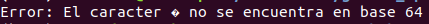
\includegraphics[scale=0.6]{images/errorArchivoBinario.png}
\caption{Resultado de las pruebas con archivos binarios}
\label{fig:errorBinario}
\end{figure}

Esto ocurre porque la codificación en base64 trabaja con un conjunto de valores correspondientes a la tabla ASCII y cuando se ingresan caracteres que no pertenecen a esta tabla no puede codificarlos y falla.


\section{Código}
\subsection{Código en C}
Ver apéndice \ref{apendice:codigo_c}

\subsection{Código assembly en MIPS32}
Ver apéndice \ref{apendice:codigo_assembly}

\section{Conclusiones}

Se realizo un programa totalmente funcional que permite la codificación de texto a Base64 y recibe instrucciones por línea de comandos, se incluyeron pruebas que corroboran la validez del código y se logró obtener el código assembly específico de la arquitectura MIPS. Esto permitió el entendimiento de herramientas necesarias por la cátedra así como chequear su funcionamiento. \newline

Se realizaron pruebas con archivos de texto, binarios y archivos de gran tamaño y las conclusiones son las siguientes:
\begin{itemize}
    \item Todas las pruebas con archivos de textos resultaron exitosas, se validaron los casos bordes en donde el programa era posible que fallara en la codificación y regresando los mismos archivos a su forma de texto se comprobó que la decodificación también era correcta.
    
    \item No todas las pruebas con archivos binarios resultan exitosas, en ciertos casos se obtiene un carácter que no se encuentra en la tabla de índice de base64 lo cual vuelve imposible la codificación del archivo, razón por la cual el programa lanza el error que se muestra en la figura \ref{fig:errorBinario}.
    
    \item Al realizar pruebas con grandes entradas de datos el programa funciona correctamente en la máquina host, tardando relativamente poco (menos de un minuto aproximadamente). Sin embargo, al ejecutar el mismo programa con el mismo archivo de entrada en la máquina guest (MIPS32) el mismo es muchísimo más lento, al punto que se tuvo que detener la ejecución del programa 10 minutos después de iniciar y no se pudo determinar el tiempo total de ejecución.
    
    \item Al realizar la misma prueba (de volumen) con un mega de bytes en lugar de un giga en la máquina host se obtiene un tiempo de ejecución mucho menor a la maquina guest, en esta ocasión no fue necesario detener la ejecución pues el programa dio el resultado esperado, sin embargo se puede notar como al cambiar entorno de ejecución el programa se ralentiza al punto de ser aproximadamente 27 veces más lento (2.744s -tiempo en máquina guest y 0,100s -tiempo en máquina host).
    
\end{itemize}

\newpage
\appendix
\section{Código}
\subsection{Código en C}
\label{apendice:codigo_c}
\begin{lstlisting}[style=customC]
#define _GNU_SOURCE
#include <stdio.h>
#include <stdlib.h>
#include <string.h>
#include <stddef.h>
#include <ctype.h>
#include <stdbool.h>
#define _POSIX_C_SOURCE 200809L //para incluir getline
char* BASE64 = "ABCDEFGHIJKLMNOPQRSTUVWXYZabcdefghijklmnopqrstuvwxyz0123456789+/";

void printHelp();
int combineBytes(char* block, size_t readBytes, bool code);
char* codification(int binaryCode, size_t readBytes);
char* decodification(int binaryCode, size_t readBytes);
int findPosition(char caracter);
void removeCharacter(char* buffer, char character, size_t* readBytes);
void resetBuffer(char* buffer);
void modifyBuffer(char* buffer);



int main(int argc, char const *argv[]){
	bool code = true; //flag para saber que operacion realizar
	FILE* inputFile = stdin;
	FILE* outputFile = stdout;
	char* (*func)(int, size_t) = codification;

	for (size_t i = 1; i < argc; i++){
		if (!strcmp(argv[i], "-h") || !strcmp(argv[i], "--help")) {
			printHelp();
			return 0;
		}

		else if (!strcmp(argv[i], "-V") || !strcmp(argv[i], "--version")){
			fprintf(stdout, "Version 1.0.0\n");
			return 0;
		}

		else if (!strcmp(argv[i], "-d") || !strcmp(argv[i], "--decode")){
			code = false;
			func = decodification;
		}

		else if (!strcmp(argv[i], "-i") || !strcmp(argv[i], "--input")){
			inputFile = fopen(argv[i + 1], "r");

			if(!inputFile){
					fprintf(stderr, "Error: Cannot open/find the specified input file");
					return 1;
			}
		}

		else if (!strcmp(argv[i], "-o") || !strcmp(argv[i], "--output")){
			outputFile = fopen(argv[i + 1], "w");

			if(!outputFile){
					fprintf(stderr, "Error: Cannot open/find the specified input file");
					return 1;
			}
		}
	}

	int bufferSize = (code) ? 4 : 5; // ambos estan +1 para incluir el \0
	char buffer[bufferSize];
	buffer[bufferSize - 1] = '\0';
	size_t readBytes = fread(buffer, 1, sizeof(buffer) - 1, inputFile);

	while(!feof(inputFile) || readBytes != 0){
		if (!code && (strstr(buffer, "=") || strstr(buffer, "\n"))){
			char remove = (strstr(buffer, "=")) ? '=' : '\n';
			removeCharacter(buffer, remove, &readBytes);
			if (!readBytes) break;
		}

		int combinedBytes = combineBytes(buffer, readBytes, code);
		
		if (combinedBytes < 0){
			return 1;
		}

		char* result = func(combinedBytes, readBytes);
		fwrite(result, sizeof(char), strlen(result), outputFile);
		free(result);
		resetBuffer(buffer); //Lo limpiamos para que no quede con basura en cada iteracion
		readBytes = fread(buffer, 1, sizeof(buffer) - 1, inputFile);
	}
	return 0;
}



void printHelp(){
	fprintf(stdout, "Usage:\n\ttp0 -h\n\ttp0 -V\n\ttp0 [options]\n");
	fprintf(stdout, "Options:\n\t-V, --version \tPrint version and quit.\n\t-h, --help\
	Print this information.\n\t-o, --output \tPath to output file.\n\t-i, --input\
	Path to input file.\n\t-d, --decode \tDecode a base64-encoded file.\n");
	fprintf(stdout, "Examples: \n\ttp0 -i input.txt -o output.txt\n");

}

int combineBytes(char* block, size_t readBytes, bool code){
	int resultado = (0x00000000);
	int SHIFTS = 24;
	int mult = (code) ? 8 : 6;
	for (int i = 0; i < readBytes; i++){
		int shiftLeft = SHIFTS - (i + 1) * mult;
		int toShift = (code) ? (int)block[i] : findPosition(block[i]);
		if (toShift < 0){
			fprintf(stderr, "Error: El caracter %c no se encuentra en base 64\n", block[i]);
			return -1;
		}
		resultado |= toShift << shiftLeft;
	}
	return resultado;
}


char* codification(int binaryCode, size_t readBytes){
	int shiftsLeft[] = {8, 14, 20, 26};
	int shiftRight = 26;
	char* code = malloc(5);
	code[0] = '=';
	code[1] = '=';
	code[2] = '=';
	code[3] = '=';
	code[4] = '\0';
	size_t posCode = 0;
	for (size_t i = 0; i < readBytes + 1; i++){
		int binaryCodeAux = binaryCode; //Para no modificar el codigo binario original
		binaryCodeAux = binaryCodeAux << shiftsLeft[i];
		binaryCodeAux = (int)((unsigned) binaryCodeAux >> shiftRight);
		code[posCode++] = BASE64[binaryCodeAux];
	}
	return code;
}

char* decodification(int binaryCode, size_t readBytes){
	int shiftsLeft[] = {8, 16, 24};
	int shiftRight = 24; 
	char* code = malloc(readBytes);
	code[readBytes - 1] = '\0';

	size_t posCode = 0;
	for (size_t i = 0; i < readBytes - 1; i++){
		int binaryCodeAux = binaryCode;
		binaryCodeAux = binaryCodeAux << shiftsLeft[i];
		binaryCodeAux = (int)((unsigned) binaryCodeAux >> shiftRight);
		code[posCode++] = (char) binaryCodeAux;
	}
	return code;
}

int findPosition(char caracter){
	for (int i = 0; i < strlen(BASE64); i++){
		if (caracter == BASE64[i]) return i;
	}
	return -1;
}

void removeCharacter(char* buffer, char character, size_t* readBytes){
	for (size_t i = 0; i < strlen(buffer); i++){
		if (buffer[i] == character) *readBytes -= 1;
	}
}

void resetBuffer(char* buffer){
	size_t pos = 0;
	while(buffer[pos] != '\0') buffer[pos++] = '\0';
}
\end{lstlisting}


\subsection{Código MIPS32}
\label{apendice:codigo_assembly}

\lstdefinestyle{custom_mips}{
  language=[mips]Assembler,        % choose the language of the code
  backgroundcolor=\color[HTML]{fcfbfc},
  numbers=left,                   % where to put the line-numbers
  stepnumber=1,                   % the step between two line-numbers.        
  numbersep=10pt,                  % how far the line-numbers are from the code
  frame=l,	                   % adds a frame around the code
  showspaces=false,               % show spaces adding particular underscores
  showstringspaces=false,         % underline spaces within strings
  keywordstyle=\color[HTML]{6684e1},
  stringstyle=\color[HTML]{1fad83},     % string literal style
  commentstyle=\color[HTML]{999580},
  showtabs=false,                 % show tabs within strings adding particular underscores
  tabsize=2,                      % sets default tabsize to 2 spaces
  captionpos=b,                   % sets the caption-position to bottom
  breaklines=true,                % sets automatic line breaking
  breakatwhitespace=true,         % sets if automatic breaks should only happen at whitespace
  title=\lstname,                 % show the filename of files included with \lstinputlisting;
  postbreak=\mbox{\textcolor{darkgray}{$\hookrightarrow$}\space},
}

\begin{lstlisting}[style=custom_mips]
	.file	1 "tp0.c"
	.section .mdebug.abi32
	.previous
	.nan	legacy
	.module	fp=xx
	.module	nooddspreg
	.abicalls
	.globl	BASE64
	.rdata
	.align	2
$LC0:
	.ascii	"ABCDEFGHIJKLMNOPQRSTUVWXYZabcdefghijklmnopqrstuvwxyz0123"
	.ascii	"456789+/\000"
	.section	.data.rel.local,"aw",@progbits
	.align	2
	.type	BASE64, @object
	.size	BASE64, 4
BASE64:
	.word	$LC0
	.rdata
	.align	2
$LC1:
	.ascii	"-h\000"
	.align	2
$LC2:
	.ascii	"--help\000"
	.align	2
$LC3:
	.ascii	"-V\000"
	.align	2
$LC4:
	.ascii	"--version\000"
	.align	2
$LC5:
	.ascii	"Version 1.0.0\012\000"
	.align	2
$LC6:
	.ascii	"-d\000"
	.align	2
$LC7:
	.ascii	"--decode\000"
	.align	2
$LC8:
	.ascii	"-i\000"
	.align	2
$LC9:
	.ascii	"--input\000"
	.align	2
$LC10:
	.ascii	"r\000"
	.align	2
$LC11:
	.ascii	"Error: Cannot open/find the specified input file\000"
	.align	2
$LC12:
	.ascii	"-o\000"
	.align	2
$LC13:
	.ascii	"--output\000"
	.align	2
$LC14:
	.ascii	"w\000"
	.text
	.align	2
	.globl	main
	.set	nomips16
	.set	nomicromips
	.ent	main
	.type	main, @function
main:
	.frame	$fp,120,$31		# vars= 56, regs= 10/0, args= 16, gp= 8
	.mask	0xc0ff0000,-4
	.fmask	0x00000000,0
	.set	noreorder
	.cpload	$25
	.set	nomacro
	addiu	$sp,$sp,-120
	sw	$31,116($sp)
	sw	$fp,112($sp)
	sw	$23,108($sp)
	sw	$22,104($sp)
	sw	$21,100($sp)
	sw	$20,96($sp)
	sw	$19,92($sp)
	sw	$18,88($sp)
	sw	$17,84($sp)
	sw	$16,80($sp)
	move	$fp,$sp
	.cprestore	16
	sw	$4,120($fp)
	sw	$5,124($fp)
	li	$2,1			# 0x1
	sb	$2,24($fp)
	lw	$2,%got(stdin)($28)
	lw	$2,0($2)
	sw	$2,28($fp)
	lw	$2,%got(stdout)($28)
	lw	$2,0($2)
	sw	$2,32($fp)
	lw	$2,%got(codification)($28)
	sw	$2,36($fp)
	li	$2,1			# 0x1
	sw	$2,40($fp)
	b	$L2
	nop

$L15:
	lw	$2,40($fp)
	sll	$2,$2,2
	lw	$3,124($fp)
	addu	$2,$3,$2
	lw	$3,0($2)
	lw	$2,%got($LC1)($28)
	addiu	$5,$2,%lo($LC1)
	move	$4,$3
	lw	$2,%call16(strcmp)($28)
	move	$25,$2
	.reloc	1f,R_MIPS_JALR,strcmp
1:	jalr	$25
	nop

	lw	$28,16($fp)
	beq	$2,$0,$L3
	nop

	lw	$2,40($fp)
	sll	$2,$2,2
	lw	$3,124($fp)
	addu	$2,$3,$2
	lw	$3,0($2)
	lw	$2,%got($LC2)($28)
	addiu	$5,$2,%lo($LC2)
	move	$4,$3
	lw	$2,%call16(strcmp)($28)
	move	$25,$2
	.reloc	1f,R_MIPS_JALR,strcmp
1:	jalr	$25
	nop

	lw	$28,16($fp)
	bne	$2,$0,$L4
	nop

$L3:
	lw	$2,%got(printHelp)($28)
	move	$25,$2
	.reloc	1f,R_MIPS_JALR,printHelp
1:	jalr	$25
	nop

	lw	$28,16($fp)
	move	$2,$0
	b	$L27
	nop

$L4:
	lw	$2,40($fp)
	sll	$2,$2,2
	lw	$3,124($fp)
	addu	$2,$3,$2
	lw	$3,0($2)
	lw	$2,%got($LC3)($28)
	addiu	$5,$2,%lo($LC3)
	move	$4,$3
	lw	$2,%call16(strcmp)($28)
	move	$25,$2
	.reloc	1f,R_MIPS_JALR,strcmp
1:	jalr	$25
	nop

	lw	$28,16($fp)
	beq	$2,$0,$L6
	nop

	lw	$2,40($fp)
	sll	$2,$2,2
	lw	$3,124($fp)
	addu	$2,$3,$2
	lw	$3,0($2)
	lw	$2,%got($LC4)($28)
	addiu	$5,$2,%lo($LC4)
	move	$4,$3
	lw	$2,%call16(strcmp)($28)
	move	$25,$2
	.reloc	1f,R_MIPS_JALR,strcmp
1:	jalr	$25
	nop

	lw	$28,16($fp)
	bne	$2,$0,$L7
	nop

$L6:
	lw	$2,%got(stdout)($28)
	lw	$2,0($2)
	move	$7,$2
	li	$6,14			# 0xe
	li	$5,1			# 0x1
	lw	$2,%got($LC5)($28)
	addiu	$4,$2,%lo($LC5)
	lw	$2,%call16(fwrite)($28)
	move	$25,$2
	.reloc	1f,R_MIPS_JALR,fwrite
1:	jalr	$25
	nop

	lw	$28,16($fp)
	move	$2,$0
	b	$L27
	nop

$L7:
	lw	$2,40($fp)
	sll	$2,$2,2
	lw	$3,124($fp)
	addu	$2,$3,$2
	lw	$3,0($2)
	lw	$2,%got($LC6)($28)
	addiu	$5,$2,%lo($LC6)
	move	$4,$3
	lw	$2,%call16(strcmp)($28)
	move	$25,$2
	.reloc	1f,R_MIPS_JALR,strcmp
1:	jalr	$25
	nop

	lw	$28,16($fp)
	beq	$2,$0,$L8
	nop

	lw	$2,40($fp)
	sll	$2,$2,2
	lw	$3,124($fp)
	addu	$2,$3,$2
	lw	$3,0($2)
	lw	$2,%got($LC7)($28)
	addiu	$5,$2,%lo($LC7)
	move	$4,$3
	lw	$2,%call16(strcmp)($28)
	move	$25,$2
	.reloc	1f,R_MIPS_JALR,strcmp
1:	jalr	$25
	nop

	lw	$28,16($fp)
	bne	$2,$0,$L9
	nop

$L8:
	sb	$0,24($fp)
	lw	$2,%got(decodification)($28)
	sw	$2,36($fp)
	b	$L10
	nop

$L9:
	lw	$2,40($fp)
	sll	$2,$2,2
	lw	$3,124($fp)
	addu	$2,$3,$2
	lw	$3,0($2)
	lw	$2,%got($LC8)($28)
	addiu	$5,$2,%lo($LC8)
	move	$4,$3
	lw	$2,%call16(strcmp)($28)
	move	$25,$2
	.reloc	1f,R_MIPS_JALR,strcmp
1:	jalr	$25
	nop

	lw	$28,16($fp)
	beq	$2,$0,$L11
	nop

	lw	$2,40($fp)
	sll	$2,$2,2
	lw	$3,124($fp)
	addu	$2,$3,$2
	lw	$3,0($2)
	lw	$2,%got($LC9)($28)
	addiu	$5,$2,%lo($LC9)
	move	$4,$3
	lw	$2,%call16(strcmp)($28)
	move	$25,$2
	.reloc	1f,R_MIPS_JALR,strcmp
1:	jalr	$25
	nop

	lw	$28,16($fp)
	bne	$2,$0,$L12
	nop

$L11:
	lw	$2,40($fp)
	addiu	$2,$2,1
	sll	$2,$2,2
	lw	$3,124($fp)
	addu	$2,$3,$2
	lw	$3,0($2)
	lw	$2,%got($LC10)($28)
	addiu	$5,$2,%lo($LC10)
	move	$4,$3
	lw	$2,%call16(fopen)($28)
	move	$25,$2
	.reloc	1f,R_MIPS_JALR,fopen
1:	jalr	$25
	nop

	lw	$28,16($fp)
	sw	$2,28($fp)
	lw	$2,28($fp)
	bne	$2,$0,$L10
	nop

	lw	$2,%got(stderr)($28)
	lw	$2,0($2)
	move	$7,$2
	li	$6,48			# 0x30
	li	$5,1			# 0x1
	lw	$2,%got($LC11)($28)
	addiu	$4,$2,%lo($LC11)
	lw	$2,%call16(fwrite)($28)
	move	$25,$2
	.reloc	1f,R_MIPS_JALR,fwrite
1:	jalr	$25
	nop

	lw	$28,16($fp)
	li	$2,1			# 0x1
	b	$L27
	nop

$L12:
	lw	$2,40($fp)
	sll	$2,$2,2
	lw	$3,124($fp)
	addu	$2,$3,$2
	lw	$3,0($2)
	lw	$2,%got($LC12)($28)
	addiu	$5,$2,%lo($LC12)
	move	$4,$3
	lw	$2,%call16(strcmp)($28)
	move	$25,$2
	.reloc	1f,R_MIPS_JALR,strcmp
1:	jalr	$25
	nop

	lw	$28,16($fp)
	beq	$2,$0,$L14
	nop

	lw	$2,40($fp)
	sll	$2,$2,2
	lw	$3,124($fp)
	addu	$2,$3,$2
	lw	$3,0($2)
	lw	$2,%got($LC13)($28)
	addiu	$5,$2,%lo($LC13)
	move	$4,$3
	lw	$2,%call16(strcmp)($28)
	move	$25,$2
	.reloc	1f,R_MIPS_JALR,strcmp
1:	jalr	$25
	nop

	lw	$28,16($fp)
	bne	$2,$0,$L10
	nop

$L14:
	lw	$2,40($fp)
	addiu	$2,$2,1
	sll	$2,$2,2
	lw	$3,124($fp)
	addu	$2,$3,$2
	lw	$3,0($2)
	lw	$2,%got($LC14)($28)
	addiu	$5,$2,%lo($LC14)
	move	$4,$3
	lw	$2,%call16(fopen)($28)
	move	$25,$2
	.reloc	1f,R_MIPS_JALR,fopen
1:	jalr	$25
	nop

	lw	$28,16($fp)
	sw	$2,32($fp)
	lw	$2,32($fp)
	bne	$2,$0,$L10
	nop

	lw	$2,%got(stderr)($28)
	lw	$2,0($2)
	move	$7,$2
	li	$6,48			# 0x30
	li	$5,1			# 0x1
	lw	$2,%got($LC11)($28)
	addiu	$4,$2,%lo($LC11)
	lw	$2,%call16(fwrite)($28)
	move	$25,$2
	.reloc	1f,R_MIPS_JALR,fwrite
1:	jalr	$25
	nop

	lw	$28,16($fp)
	li	$2,1			# 0x1
	b	$L27
	nop

$L10:
	lw	$2,40($fp)
	addiu	$2,$2,1
	sw	$2,40($fp)
$L2:
	lw	$2,120($fp)
	lw	$3,40($fp)
	sltu	$2,$3,$2
	bne	$2,$0,$L15
	nop

	lbu	$2,24($fp)
	beq	$2,$0,$L16
	nop

	li	$2,4			# 0x4
	b	$L17
	nop

$L16:
	li	$2,5			# 0x5
$L17:
	sw	$2,44($fp)
	lw	$2,44($fp)
	move	$4,$2
	sw	$4,72($fp)
	move	$2,$sp
	sw	$2,76($fp)
	move	$2,$4
	addiu	$2,$2,-1
	sw	$2,48($fp)
	move	$2,$4
	move	$23,$2
	move	$22,$0
	srl	$2,$23,29
	sll	$18,$22,3
	or	$18,$2,$18
	sll	$19,$23,3
	move	$2,$4
	move	$21,$2
	move	$20,$0
	srl	$2,$21,29
	sll	$16,$20,3
	or	$16,$2,$16
	sll	$17,$21,3
	move	$2,$4
	addiu	$2,$2,7
	srl	$2,$2,3
	sll	$2,$2,3
	subu	$sp,$sp,$2
	addiu	$2,$sp,16
	addiu	$2,$2,0
	sw	$2,52($fp)
	lw	$2,44($fp)
	addiu	$2,$2,-1
	lw	$3,52($fp)
	addu	$2,$3,$2
	sb	$0,0($2)
	lw	$2,52($fp)
	move	$3,$4
	addiu	$3,$3,-1
	lw	$7,28($fp)
	move	$6,$3
	li	$5,1			# 0x1
	move	$4,$2
	lw	$2,%call16(fread)($28)
	move	$25,$2
	.reloc	1f,R_MIPS_JALR,fread
1:	jalr	$25
	nop

	lw	$28,16($fp)
	sw	$2,68($fp)
	b	$L18
	nop

$L26:
	lbu	$2,24($fp)
	xori	$2,$2,0x1
	andi	$2,$2,0x00ff
	beq	$2,$0,$L19
	nop

	lw	$2,52($fp)
	li	$5,61			# 0x3d
	move	$4,$2
	lw	$2,%call16(strchr)($28)
	move	$25,$2
	.reloc	1f,R_MIPS_JALR,strchr
1:	jalr	$25
	nop

	lw	$28,16($fp)
	bne	$2,$0,$L20
	nop

	lw	$2,52($fp)
	li	$5,10			# 0xa
	move	$4,$2
	lw	$2,%call16(strchr)($28)
	move	$25,$2
	.reloc	1f,R_MIPS_JALR,strchr
1:	jalr	$25
	nop

	lw	$28,16($fp)
	beq	$2,$0,$L19
	nop

$L20:
	lw	$2,52($fp)
	li	$5,61			# 0x3d
	move	$4,$2
	lw	$2,%call16(strchr)($28)
	move	$25,$2
	.reloc	1f,R_MIPS_JALR,strchr
1:	jalr	$25
	nop

	lw	$28,16($fp)
	beq	$2,$0,$L21
	nop

	li	$2,61			# 0x3d
	b	$L22
	nop

$L21:
	li	$2,10			# 0xa
$L22:
	sb	$2,56($fp)
	lw	$2,52($fp)
	addiu	$4,$fp,68
	lb	$3,56($fp)
	move	$6,$4
	move	$5,$3
	move	$4,$2
	lw	$2,%got(removeCharacter)($28)
	move	$25,$2
	.reloc	1f,R_MIPS_JALR,removeCharacter
1:	jalr	$25
	nop

	lw	$28,16($fp)
	lw	$2,68($fp)
	beq	$2,$0,$L28
	nop

$L19:
	lw	$2,52($fp)
	lw	$3,68($fp)
	lbu	$4,24($fp)
	move	$6,$4
	move	$5,$3
	move	$4,$2
	lw	$2,%got(combineBytes)($28)
	move	$25,$2
	.reloc	1f,R_MIPS_JALR,combineBytes
1:	jalr	$25
	nop

	lw	$28,16($fp)
	sw	$2,60($fp)
	lw	$2,60($fp)
	bgez	$2,$L24
	nop

	li	$2,1			# 0x1
	b	$L25
	nop

$L24:
	lw	$3,68($fp)
	lw	$2,36($fp)
	move	$5,$3
	lw	$4,60($fp)
	move	$25,$2
	jalr	$25
	nop

	lw	$28,16($fp)
	sw	$2,64($fp)
	lw	$4,64($fp)
	lw	$2,%call16(strlen)($28)
	move	$25,$2
	.reloc	1f,R_MIPS_JALR,strlen
1:	jalr	$25
	nop

	lw	$28,16($fp)
	lw	$7,32($fp)
	move	$6,$2
	li	$5,1			# 0x1
	lw	$4,64($fp)
	lw	$2,%call16(fwrite)($28)
	move	$25,$2
	.reloc	1f,R_MIPS_JALR,fwrite
1:	jalr	$25
	nop

	lw	$28,16($fp)
	lw	$4,64($fp)
	lw	$2,%call16(free)($28)
	move	$25,$2
	.reloc	1f,R_MIPS_JALR,free
1:	jalr	$25
	nop

	lw	$28,16($fp)
	lw	$2,52($fp)
	move	$4,$2
	lw	$2,%got(resetBuffer)($28)
	move	$25,$2
	.reloc	1f,R_MIPS_JALR,resetBuffer
1:	jalr	$25
	nop

	lw	$28,16($fp)
	lw	$2,52($fp)
	lw	$3,72($fp)
	addiu	$3,$3,-1
	lw	$7,28($fp)
	move	$6,$3
	li	$5,1			# 0x1
	move	$4,$2
	lw	$2,%call16(fread)($28)
	move	$25,$2
	.reloc	1f,R_MIPS_JALR,fread
1:	jalr	$25
	nop

	lw	$28,16($fp)
	sw	$2,68($fp)
$L18:
	lw	$4,28($fp)
	lw	$2,%call16(feof)($28)
	move	$25,$2
	.reloc	1f,R_MIPS_JALR,feof
1:	jalr	$25
	nop

	lw	$28,16($fp)
	beq	$2,$0,$L26
	nop

	lw	$2,68($fp)
	bne	$2,$0,$L26
	nop

	b	$L23
	nop

$L28:
	nop
$L23:
	move	$2,$0
$L25:
	lw	$sp,76($fp)
$L27:
	move	$sp,$fp
	lw	$31,116($sp)
	lw	$fp,112($sp)
	lw	$23,108($sp)
	lw	$22,104($sp)
	lw	$21,100($sp)
	lw	$20,96($sp)
	lw	$19,92($sp)
	lw	$18,88($sp)
	lw	$17,84($sp)
	lw	$16,80($sp)
	addiu	$sp,$sp,120
	jr	$31
	nop

	.set	macro
	.set	reorder
	.end	main
	.size	main, .-main
	.rdata
	.align	2
$LC15:
	.ascii	"Usage:\012\011tp0 -h\012\011tp0 -V\012\011tp0 [options]\012"
	.ascii	"\000"
	.align	2
$LC16:
	.ascii	"Options:\012\011-V, --version \011Print version and quit"
	.ascii	".\012\011-h, --help\011Print this information.\012\011-o"
	.ascii	", --output \011Path to output file.\012\011-i, --input\011"
	.ascii	"Path to input file.\012\011-d, --decode \011Decode a bas"
	.ascii	"e64-encoded file.\012\000"
	.align	2
$LC17:
	.ascii	"Examples: \012\011tp0 -i input.txt -o output.txt\012\000"
	.text
	.align	2
	.globl	printHelp
	.set	nomips16
	.set	nomicromips
	.ent	printHelp
	.type	printHelp, @function
printHelp:
	.frame	$fp,32,$31		# vars= 0, regs= 2/0, args= 16, gp= 8
	.mask	0xc0000000,-4
	.fmask	0x00000000,0
	.set	noreorder
	.cpload	$25
	.set	nomacro
	addiu	$sp,$sp,-32
	sw	$31,28($sp)
	sw	$fp,24($sp)
	move	$fp,$sp
	.cprestore	16
	lw	$2,%got(stdout)($28)
	lw	$2,0($2)
	move	$7,$2
	li	$6,38			# 0x26
	li	$5,1			# 0x1
	lw	$2,%got($LC15)($28)
	addiu	$4,$2,%lo($LC15)
	lw	$2,%call16(fwrite)($28)
	move	$25,$2
	.reloc	1f,R_MIPS_JALR,fwrite
1:	jalr	$25
	nop

	lw	$28,16($fp)
	lw	$2,%got(stdout)($28)
	lw	$2,0($2)
	move	$7,$2
	li	$6,199			# 0xc7
	li	$5,1			# 0x1
	lw	$2,%got($LC16)($28)
	addiu	$4,$2,%lo($LC16)
	lw	$2,%call16(fwrite)($28)
	move	$25,$2
	.reloc	1f,R_MIPS_JALR,fwrite
1:	jalr	$25
	nop

	lw	$28,16($fp)
	lw	$2,%got(stdout)($28)
	lw	$2,0($2)
	move	$7,$2
	li	$6,43			# 0x2b
	li	$5,1			# 0x1
	lw	$2,%got($LC17)($28)
	addiu	$4,$2,%lo($LC17)
	lw	$2,%call16(fwrite)($28)
	move	$25,$2
	.reloc	1f,R_MIPS_JALR,fwrite
1:	jalr	$25
	nop

	lw	$28,16($fp)
	nop
	move	$sp,$fp
	lw	$31,28($sp)
	lw	$fp,24($sp)
	addiu	$sp,$sp,32
	jr	$31
	nop

	.set	macro
	.set	reorder
	.end	printHelp
	.size	printHelp, .-printHelp
	.rdata
	.align	2
$LC18:
	.ascii	"Error: El caracter %c no se encuentra en base 64\012\000"
	.text
	.align	2
	.globl	combineBytes
	.set	nomips16
	.set	nomicromips
	.ent	combineBytes
	.type	combineBytes, @function
combineBytes:
	.frame	$fp,56,$31		# vars= 24, regs= 2/0, args= 16, gp= 8
	.mask	0xc0000000,-4
	.fmask	0x00000000,0
	.set	noreorder
	.cpload	$25
	.set	nomacro
	addiu	$sp,$sp,-56
	sw	$31,52($sp)
	sw	$fp,48($sp)
	move	$fp,$sp
	.cprestore	16
	sw	$4,56($fp)
	sw	$5,60($fp)
	move	$2,$6
	sb	$2,64($fp)
	sw	$0,24($fp)
	li	$2,24			# 0x18
	sw	$2,32($fp)
	lbu	$2,64($fp)
	beq	$2,$0,$L31
	nop

	li	$2,8			# 0x8
	b	$L32
	nop

$L31:
	li	$2,6			# 0x6
$L32:
	sw	$2,36($fp)
	sw	$0,28($fp)
	b	$L33
	nop

$L38:
	lw	$2,28($fp)
	addiu	$3,$2,1
	lw	$2,36($fp)
	mul	$2,$3,$2
	lw	$3,32($fp)
	subu	$2,$3,$2
	sw	$2,40($fp)
	lbu	$2,64($fp)
	beq	$2,$0,$L34
	nop

	lw	$2,28($fp)
	lw	$3,56($fp)
	addu	$2,$3,$2
	lb	$2,0($2)
	b	$L35
	nop

$L34:
	lw	$2,28($fp)
	lw	$3,56($fp)
	addu	$2,$3,$2
	lb	$2,0($2)
	move	$4,$2
	lw	$2,%got(findPosition)($28)
	move	$25,$2
	.reloc	1f,R_MIPS_JALR,findPosition
1:	jalr	$25
	nop

	lw	$28,16($fp)
$L35:
	sw	$2,44($fp)
	lw	$2,44($fp)
	bgez	$2,$L36
	nop

	lw	$2,%got(stderr)($28)
	lw	$4,0($2)
	lw	$2,28($fp)
	lw	$3,56($fp)
	addu	$2,$3,$2
	lb	$2,0($2)
	move	$6,$2
	lw	$2,%got($LC18)($28)
	addiu	$5,$2,%lo($LC18)
	lw	$2,%call16(fprintf)($28)
	move	$25,$2
	.reloc	1f,R_MIPS_JALR,fprintf
1:	jalr	$25
	nop

	lw	$28,16($fp)
	li	$2,-1			# 0xffffffffffffffff
	b	$L37
	nop

$L36:
	lw	$3,44($fp)
	lw	$2,40($fp)
	sll	$2,$3,$2
	lw	$3,24($fp)
	or	$2,$3,$2
	sw	$2,24($fp)
	lw	$2,28($fp)
	addiu	$2,$2,1
	sw	$2,28($fp)
$L33:
	lw	$3,28($fp)
	lw	$2,60($fp)
	sltu	$2,$3,$2
	bne	$2,$0,$L38
	nop

	lw	$2,24($fp)
$L37:
	move	$sp,$fp
	lw	$31,52($sp)
	lw	$fp,48($sp)
	addiu	$sp,$sp,56
	jr	$31
	nop

	.set	macro
	.set	reorder
	.end	combineBytes
	.size	combineBytes, .-combineBytes
	.align	2
	.globl	codification
	.set	nomips16
	.set	nomicromips
	.ent	codification
	.type	codification, @function
codification:
	.frame	$fp,72,$31		# vars= 40, regs= 2/0, args= 16, gp= 8
	.mask	0xc0000000,-4
	.fmask	0x00000000,0
	.set	noreorder
	.cpload	$25
	.set	nomacro
	addiu	$sp,$sp,-72
	sw	$31,68($sp)
	sw	$fp,64($sp)
	move	$fp,$sp
	.cprestore	16
	sw	$4,72($fp)
	sw	$5,76($fp)
	li	$2,8			# 0x8
	sw	$2,44($fp)
	li	$2,14			# 0xe
	sw	$2,48($fp)
	li	$2,20			# 0x14
	sw	$2,52($fp)
	li	$2,26			# 0x1a
	sw	$2,56($fp)
	li	$2,26			# 0x1a
	sw	$2,32($fp)
	li	$4,5			# 0x5
	lw	$2,%call16(malloc)($28)
	move	$25,$2
	.reloc	1f,R_MIPS_JALR,malloc
1:	jalr	$25
	nop

	lw	$28,16($fp)
	sw	$2,36($fp)
	lw	$2,36($fp)
	li	$3,61			# 0x3d
	sb	$3,0($2)
	lw	$2,36($fp)
	addiu	$2,$2,1
	li	$3,61			# 0x3d
	sb	$3,0($2)
	lw	$2,36($fp)
	addiu	$2,$2,2
	li	$3,61			# 0x3d
	sb	$3,0($2)
	lw	$2,36($fp)
	addiu	$2,$2,3
	li	$3,61			# 0x3d
	sb	$3,0($2)
	lw	$2,36($fp)
	addiu	$2,$2,4
	sb	$0,0($2)
	sw	$0,24($fp)
	sw	$0,28($fp)
	b	$L40
	nop

$L41:
	lw	$2,72($fp)
	sw	$2,40($fp)
	lw	$2,28($fp)
	sll	$2,$2,2
	addiu	$3,$fp,24
	addu	$2,$3,$2
	lw	$2,20($2)
	lw	$3,40($fp)
	sll	$2,$3,$2
	sw	$2,40($fp)
	lw	$3,40($fp)
	lw	$2,32($fp)
	srl	$2,$3,$2
	sw	$2,40($fp)
	lw	$2,24($fp)
	addiu	$3,$2,1
	sw	$3,24($fp)
	lw	$3,36($fp)
	addu	$2,$3,$2
	lw	$3,%got(BASE64)($28)
	lw	$4,0($3)
	lw	$3,40($fp)
	addu	$3,$4,$3
	lb	$3,0($3)
	sb	$3,0($2)
	lw	$2,28($fp)
	addiu	$2,$2,1
	sw	$2,28($fp)
$L40:
	lw	$2,76($fp)
	addiu	$3,$2,1
	lw	$2,28($fp)
	sltu	$2,$2,$3
	bne	$2,$0,$L41
	nop

	lw	$2,36($fp)
	move	$sp,$fp
	lw	$31,68($sp)
	lw	$fp,64($sp)
	addiu	$sp,$sp,72
	jr	$31
	nop

	.set	macro
	.set	reorder
	.end	codification
	.size	codification, .-codification
	.align	2
	.globl	decodification
	.set	nomips16
	.set	nomicromips
	.ent	decodification
	.type	decodification, @function
decodification:
	.frame	$fp,64,$31		# vars= 32, regs= 2/0, args= 16, gp= 8
	.mask	0xc0000000,-4
	.fmask	0x00000000,0
	.set	noreorder
	.cpload	$25
	.set	nomacro
	addiu	$sp,$sp,-64
	sw	$31,60($sp)
	sw	$fp,56($sp)
	move	$fp,$sp
	.cprestore	16
	sw	$4,64($fp)
	sw	$5,68($fp)
	li	$2,8			# 0x8
	sw	$2,44($fp)
	li	$2,16			# 0x10
	sw	$2,48($fp)
	li	$2,24			# 0x18
	sw	$2,52($fp)
	li	$2,24			# 0x18
	sw	$2,32($fp)
	lw	$4,68($fp)
	lw	$2,%call16(malloc)($28)
	move	$25,$2
	.reloc	1f,R_MIPS_JALR,malloc
1:	jalr	$25
	nop

	lw	$28,16($fp)
	sw	$2,36($fp)
	lw	$2,68($fp)
	addiu	$2,$2,-1
	lw	$3,36($fp)
	addu	$2,$3,$2
	sb	$0,0($2)
	sw	$0,24($fp)
	sw	$0,28($fp)
	b	$L44
	nop

$L45:
	lw	$2,64($fp)
	sw	$2,40($fp)
	lw	$2,28($fp)
	sll	$2,$2,2
	addiu	$3,$fp,24
	addu	$2,$3,$2
	lw	$2,20($2)
	lw	$3,40($fp)
	sll	$2,$3,$2
	sw	$2,40($fp)
	lw	$3,40($fp)
	lw	$2,32($fp)
	srl	$2,$3,$2
	sw	$2,40($fp)
	lw	$2,24($fp)
	addiu	$3,$2,1
	sw	$3,24($fp)
	lw	$3,36($fp)
	addu	$2,$3,$2
	lw	$3,40($fp)
	seb	$3,$3
	sb	$3,0($2)
	lw	$2,28($fp)
	addiu	$2,$2,1
	sw	$2,28($fp)
$L44:
	lw	$2,68($fp)
	addiu	$3,$2,-1
	lw	$2,28($fp)
	sltu	$2,$2,$3
	bne	$2,$0,$L45
	nop

	lw	$2,36($fp)
	move	$sp,$fp
	lw	$31,60($sp)
	lw	$fp,56($sp)
	addiu	$sp,$sp,64
	jr	$31
	nop

	.set	macro
	.set	reorder
	.end	decodification
	.size	decodification, .-decodification
	.align	2
	.globl	findPosition
	.set	nomips16
	.set	nomicromips
	.ent	findPosition
	.type	findPosition, @function
findPosition:
	.frame	$fp,40,$31		# vars= 8, regs= 2/0, args= 16, gp= 8
	.mask	0xc0000000,-4
	.fmask	0x00000000,0
	.set	noreorder
	.cpload	$25
	.set	nomacro
	addiu	$sp,$sp,-40
	sw	$31,36($sp)
	sw	$fp,32($sp)
	move	$fp,$sp
	.cprestore	16
	move	$2,$4
	sb	$2,40($fp)
	sw	$0,24($fp)
	b	$L48
	nop

$L51:
	lw	$2,%got(BASE64)($28)
	lw	$3,0($2)
	lw	$2,24($fp)
	addu	$2,$3,$2
	lb	$2,0($2)
	lb	$3,40($fp)
	bne	$3,$2,$L49
	nop

	lw	$2,24($fp)
	b	$L50
	nop

$L49:
	lw	$2,24($fp)
	addiu	$2,$2,1
	sw	$2,24($fp)
$L48:
	lw	$2,%got(BASE64)($28)
	lw	$2,0($2)
	move	$4,$2
	lw	$2,%call16(strlen)($28)
	move	$25,$2
	.reloc	1f,R_MIPS_JALR,strlen
1:	jalr	$25
	nop

	lw	$28,16($fp)
	move	$3,$2
	lw	$2,24($fp)
	sltu	$2,$2,$3
	bne	$2,$0,$L51
	nop

	li	$2,-1			# 0xffffffffffffffff
$L50:
	move	$sp,$fp
	lw	$31,36($sp)
	lw	$fp,32($sp)
	addiu	$sp,$sp,40
	jr	$31
	nop

	.set	macro
	.set	reorder
	.end	findPosition
	.size	findPosition, .-findPosition
	.align	2
	.globl	removeCharacter
	.set	nomips16
	.set	nomicromips
	.ent	removeCharacter
	.type	removeCharacter, @function
removeCharacter:
	.frame	$fp,40,$31		# vars= 8, regs= 2/0, args= 16, gp= 8
	.mask	0xc0000000,-4
	.fmask	0x00000000,0
	.set	noreorder
	.cpload	$25
	.set	nomacro
	addiu	$sp,$sp,-40
	sw	$31,36($sp)
	sw	$fp,32($sp)
	move	$fp,$sp
	.cprestore	16
	sw	$4,40($fp)
	move	$2,$5
	sw	$6,48($fp)
	sb	$2,44($fp)
	sw	$0,24($fp)
	b	$L53
	nop

$L55:
	lw	$3,40($fp)
	lw	$2,24($fp)
	addu	$2,$3,$2
	lb	$2,0($2)
	lb	$3,44($fp)
	bne	$3,$2,$L54
	nop

	lw	$2,48($fp)
	lw	$2,0($2)
	addiu	$3,$2,-1
	lw	$2,48($fp)
	sw	$3,0($2)
$L54:
	lw	$2,24($fp)
	addiu	$2,$2,1
	sw	$2,24($fp)
$L53:
	lw	$4,40($fp)
	lw	$2,%call16(strlen)($28)
	move	$25,$2
	.reloc	1f,R_MIPS_JALR,strlen
1:	jalr	$25
	nop

	lw	$28,16($fp)
	move	$3,$2
	lw	$2,24($fp)
	sltu	$2,$2,$3
	bne	$2,$0,$L55
	nop

	nop
	move	$sp,$fp
	lw	$31,36($sp)
	lw	$fp,32($sp)
	addiu	$sp,$sp,40
	jr	$31
	nop

	.set	macro
	.set	reorder
	.end	removeCharacter
	.size	removeCharacter, .-removeCharacter
	.align	2
	.globl	resetBuffer
	.set	nomips16
	.set	nomicromips
	.ent	resetBuffer
	.type	resetBuffer, @function
resetBuffer:
	.frame	$fp,24,$31		# vars= 8, regs= 1/0, args= 0, gp= 8
	.mask	0x40000000,-4
	.fmask	0x00000000,0
	.set	noreorder
	.set	nomacro
	addiu	$sp,$sp,-24
	sw	$fp,20($sp)
	move	$fp,$sp
	sw	$4,24($fp)
	sw	$0,8($fp)
	b	$L57
	nop

$L58:
	lw	$2,8($fp)
	addiu	$3,$2,1
	sw	$3,8($fp)
	lw	$3,24($fp)
	addu	$2,$3,$2
	sb	$0,0($2)
$L57:
	lw	$3,24($fp)
	lw	$2,8($fp)
	addu	$2,$3,$2
	lb	$2,0($2)
	bne	$2,$0,$L58
	nop

	nop
	move	$sp,$fp
	lw	$fp,20($sp)
	addiu	$sp,$sp,24
	jr	$31
	nop

	.set	macro
	.set	reorder
	.end	resetBuffer
	.size	resetBuffer, .-resetBuffer
	.ident	"GCC: (Debian 6.3.0-18+deb9u1) 6.3.0 20170516"
\end{lstlisting}

% \newpage
\section{Enunciado del trabajo práctico}
% 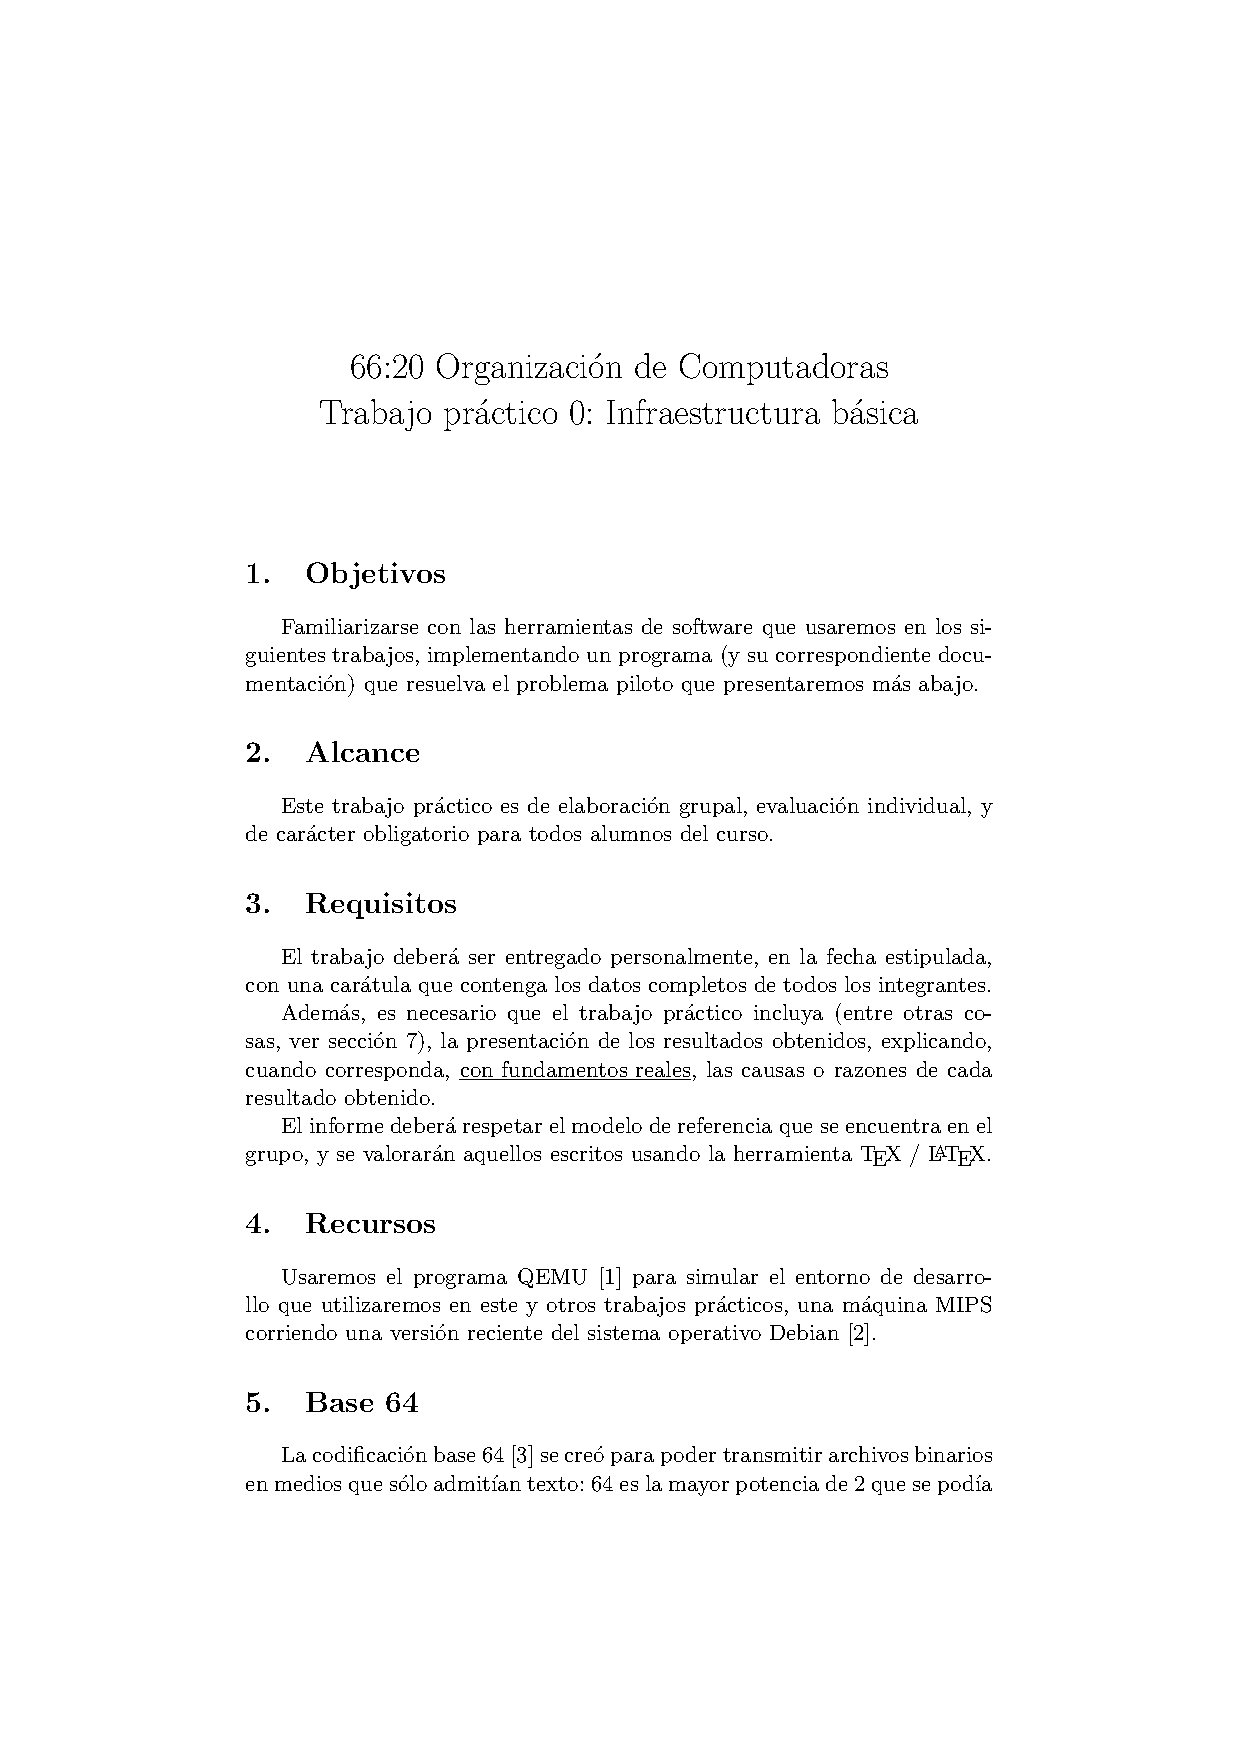
\includepdf[pages=1, scale=0.8, frame]{tp0-q2-2020.pdf}
\frame{
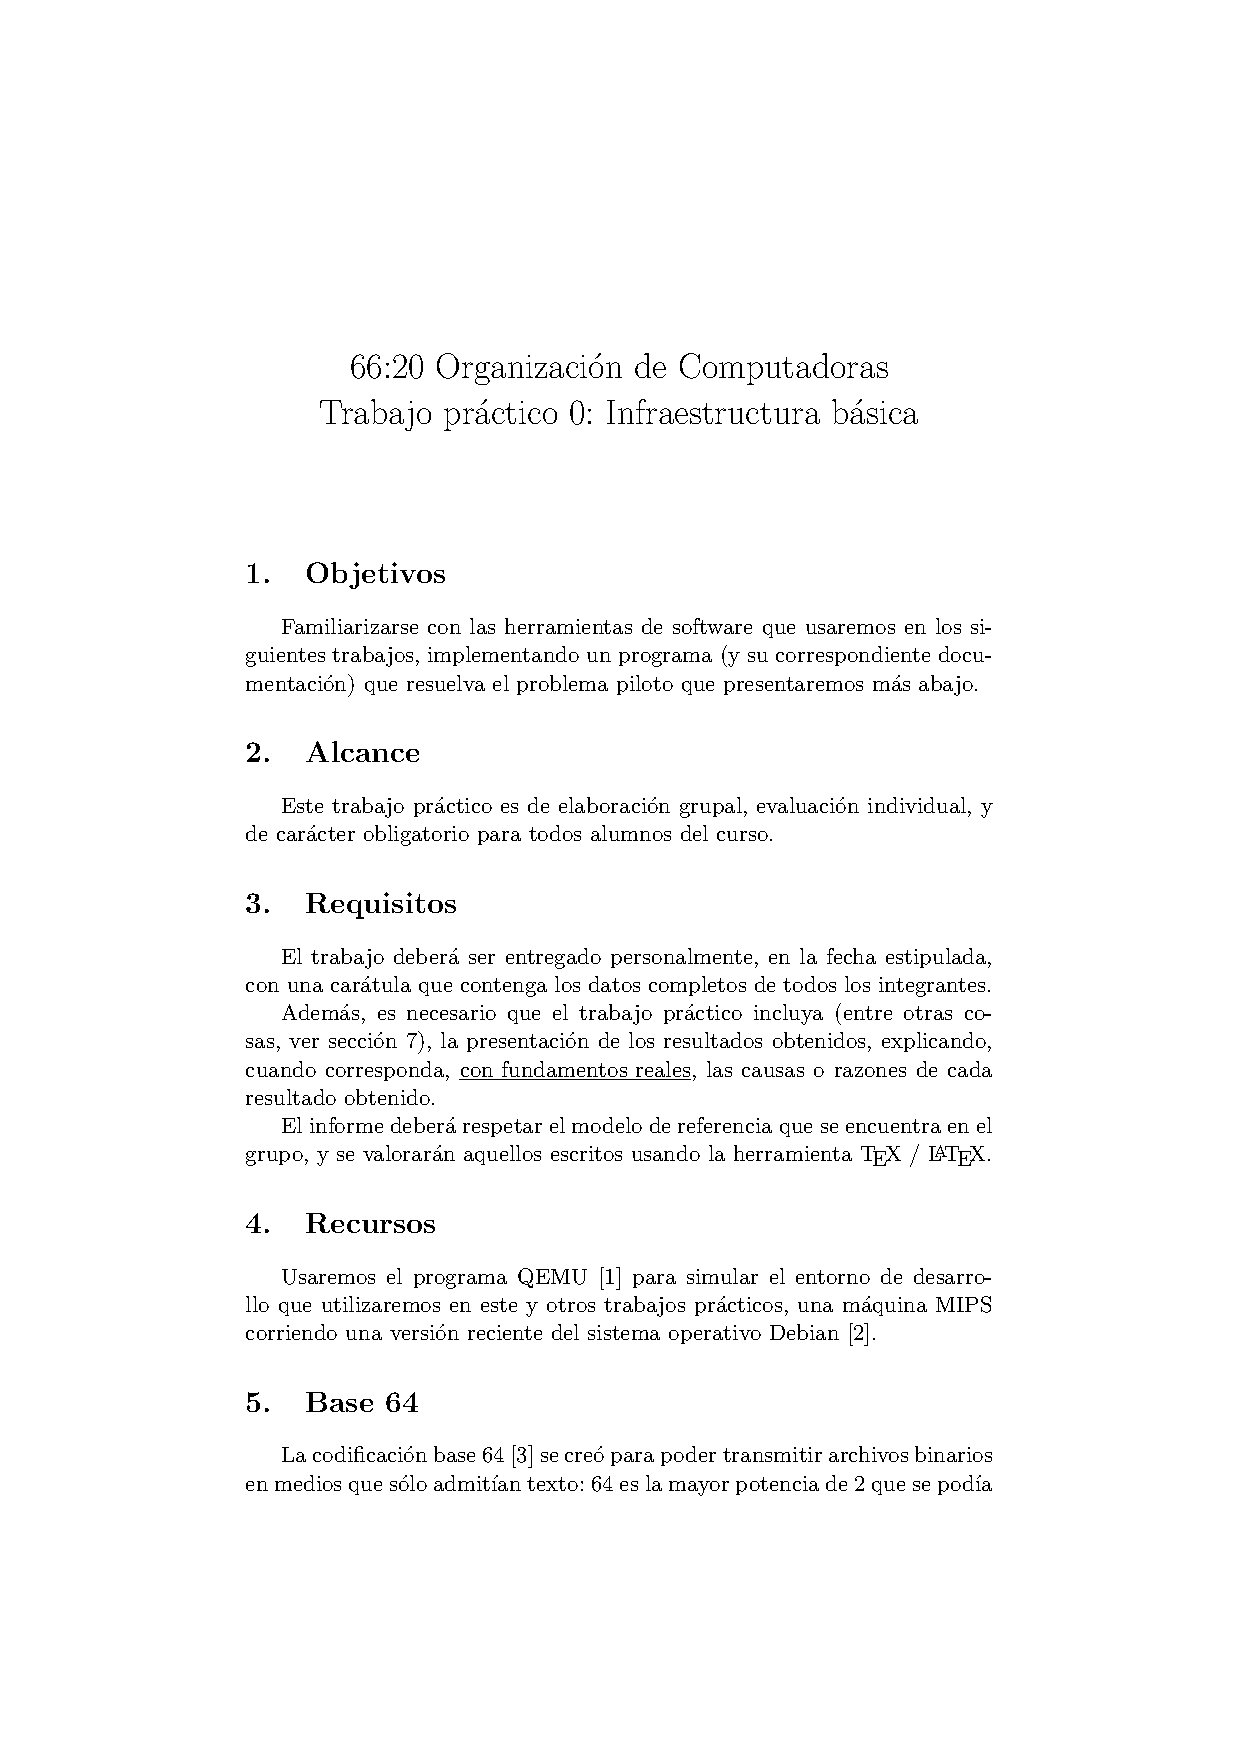
\includegraphics[height=0.93\textheight, frame]{tp0-q2-2020.pdf}
}
\includepdf[pages=2-, scale=0.8, frame]{tp0-q2-2020.pdf}
\newpage
\section{Código auxiliar}
\subsection{Pruebas automatizadas}
\label{script_python_test}
\begin{lstlisting}[language=Python]
import subprocess
import sys
import glob
import tempfile
def run_command(command):
    proc = subprocess.Popen(command, 
        stdout=subprocess.PIPE, stderr= subprocess.PIPE, 
        shell=True, universal_newlines=True)
    std_out, std_err = proc.communicate()
    return proc.returncode, std_out, std_err

def main(command, input_prefix, result_prefix):
    input_files = glob.glob(f'{input_prefix}*')
    test_files = { file_name[len(input_prefix):]: 
                    [file_name,] for file_name in input_files }
    for id, files in test_files.items():
        files.append(f'{result_prefix}{id}')
    
    for file, output_file in test_files.values():
        result_obtained = run_command(f'{command} < {file}')[1]
        with tempfile.NamedTemporaryFile() as tmp:
            tmp.write(bytes(result_obtained, encoding='utf-8'))
            tmp.read()
            code_diff, stdout_diff, _ = run_command(f"""
                diff {output_file} {tmp.name}
            """)
            if code_diff == 0:
                print('.', end='')
                continue 
            print()
            print(f'Ejecución con {file} comparación con {output_file}')
            print(stdout_diff)
            
if __name__ == "__main__":
    if len(sys.argv) == 4:
        command, input_prefix, result_prefix = sys.argv[1:]
        main(command, input_prefix, result_prefix)
    else:
        print("""
        Use: python test.py command input_prefix result_prefix
        command: comando a ejecutar.
        input_prefix: prefijo de los archivos que se usaran como entrada.
        result_prefix: prefijo de los archivos a comparar.
        """)
\end{lstlisting}

\newpage
\begin{thebibliography}{9}

\bibitem{base64}
\textit{Artículo de Wikipedia sobre Base64}. 
\href {https://es.wikipedia.org/wiki/Base64}{
https://es.wikipedia.org/wiki/Base64
}
\bibitem{ascii_table}
\textit{Tabla ascii}. 
\href {https://elcodigoascii.com.ar/}{
https://elcodigoascii.com.ar/
}
\bibitem{gcc_parameters}
\textit{Parámetros de gcc}. 
\href {https://gcc.gnu.org/onlinedocs/gcc/Option-Summary.html}{
https://gcc.gnu.org/onlinedocs/gcc/Option-Summary.html
}
\end{thebibliography}

\end{document}